\chapter{Concept}
\label{cha:Concept}

This chapter presents the conceptual approach for addressing the previously described challenges in public transportation.
It considers how a mobile application could be designed to assist users in reaching their destinations without missing their stops.

A sketched prototype serves as a reference for illustrating how such an application might be structured and what functionalities could be incorporated. 
In particular, the concept of reminder behavior is examined, exploring different triggering mechanisms and the potential use of visual, haptic and acoustic feedback to effectively notify users.
To enable these functionalities, the system would likely require the ability to store and manage essential data, such as user preferences and reminder settings. 
The possible structure and handling of this data are considered in this chapter.

\section{Prototype}
The proposed system is a mobile application, likely targeting iOS, that aims to allow commuters to plan their public transport journeys and receive reminders for their selected routes.
The idea is that users should be able to search for public transport connections by specifying a departure and arrival stop, along with the desired date and time of travel. 
Based on these inputs, the system would provide a selection of available routes, from which users can choose the most suitable option. 
Once a route is selected, a reminder mechanism is intended to ensure that users do not miss their desired destination stop. 
The idea of how such a reminder system could work is explored in more detail in Section \ref{sec:behaviour}.

The main screen of the proposed application is envisioned as the central interface for the trip planning process. 
It is structured around a selection section where the user can specify their journey details. 
At the top of this screen, two fields represent the departure and destination stops, displayed in an "A to B" format. 
Below these fields, a date and time selection is displayed with the default value set to "Depart Now", indicating immediate departure. 
Beneath this section, a search button is prominently placed, allowing users to request available public transport connections for the specified parameters.
When a user taps on either the departure or destination field, a dropdown menu is envisioned to appear, providing a list of selectable public transport stops. 
The exact filtering process for these stop suggestions is not further defined in this concept. 
However, it is anticipated that an open \ac{API} for public transport data endpoints would be required to dynamically populate the list with available stops.

If users wish to modify their departure time, tapping on the "Depart Now" button is expected to open a selection screen that slides up from the bottom of the screen, allowing them to specify a custom date and time. 
Once all trip planning parameters have been set, the system should search for available public transport routes matching the user's request.
The results screen displays the retrieved connections in a structured format. 
Each entry should present departure and arrival times, the transport service's identification (such as the line number or train designation) and the duration of the trip.
From this list, users should be able to select a preferred route, after which the reminder system will be activated for their journey.
The sketched prototype in Figure \ref{fig:prototype} provides a visual representation of this envisioned process.

\begin{figure}[htbp]
    \centering
    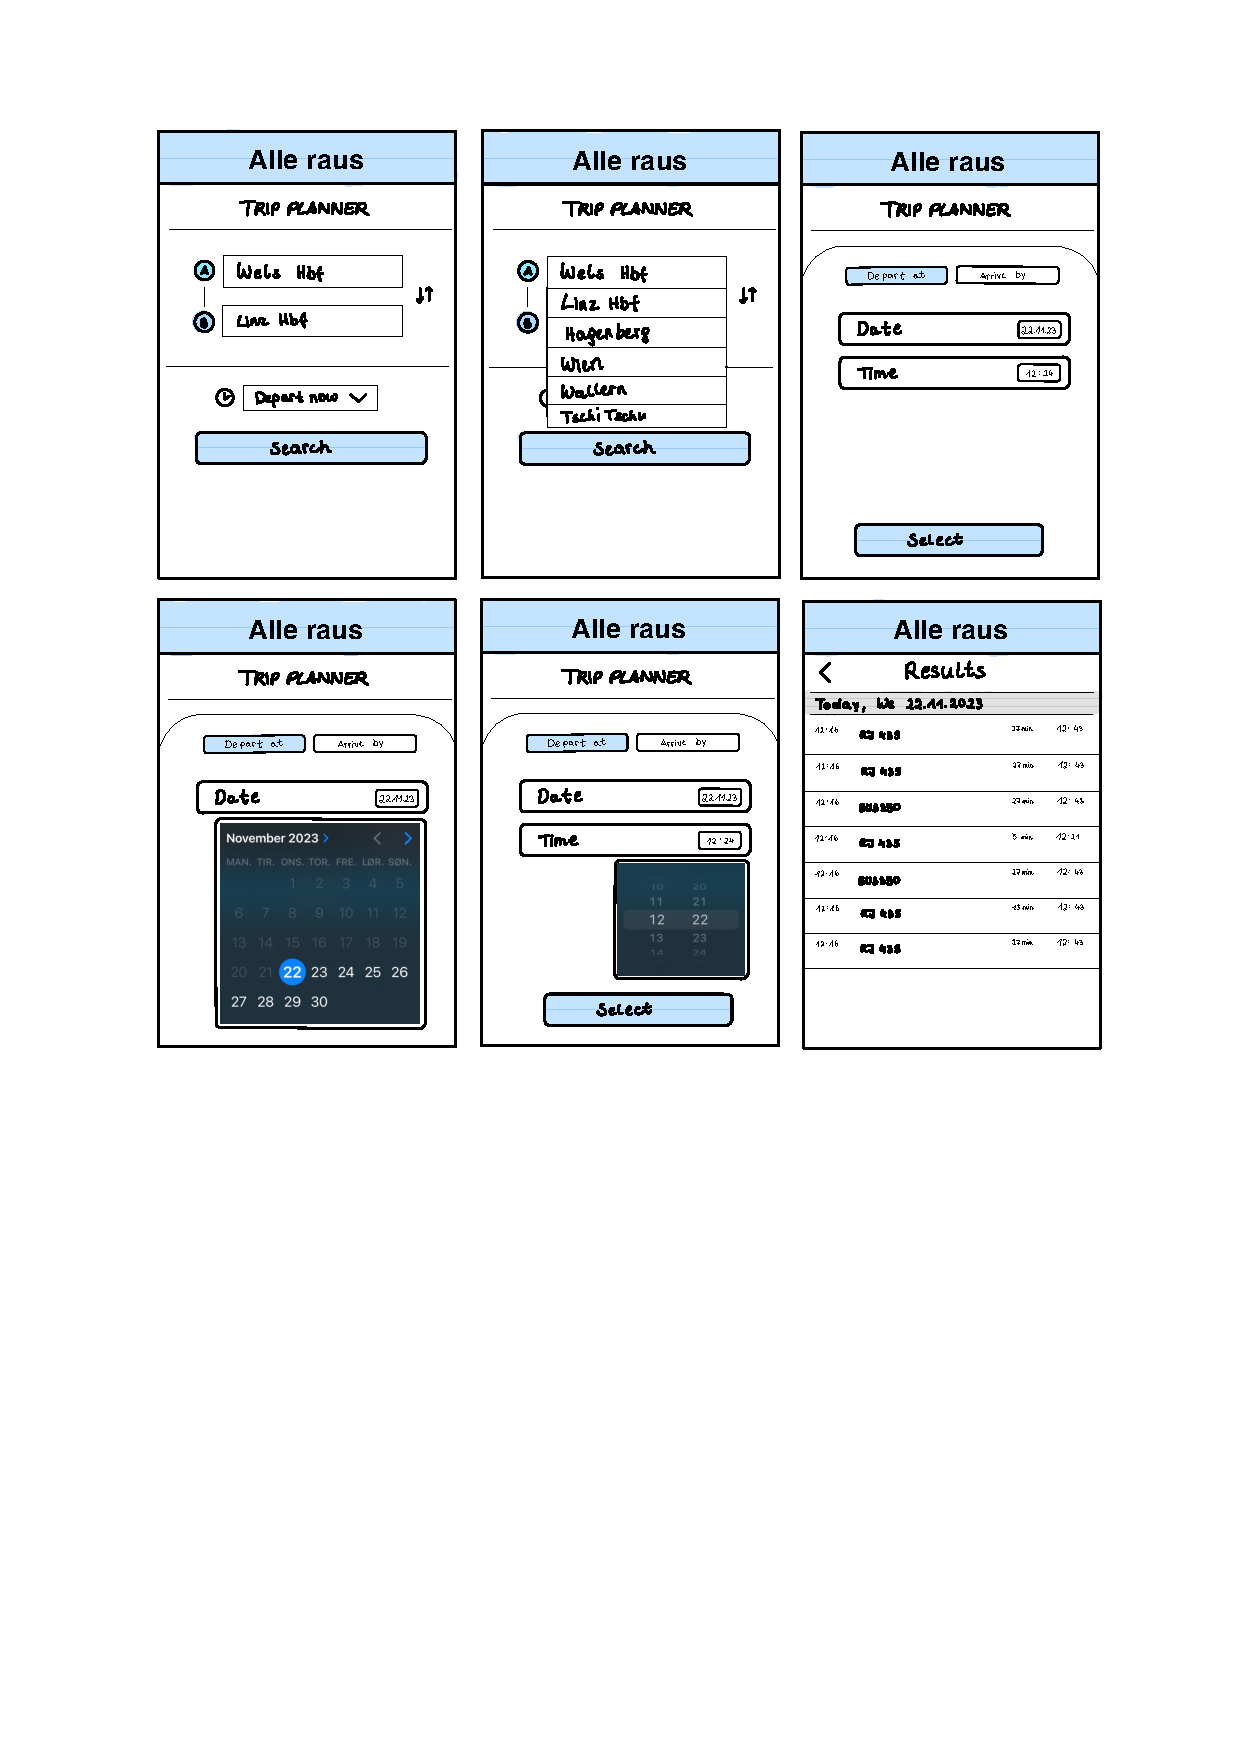
\includegraphics[width=0.9\textwidth]{Prototype.pdf}
    \caption{Prototype of a reminder app for public transportation}
    \label{fig:prototype}
\end{figure}

\section{Reminder Behaviour}
\label{sec:behaviour}
Once a user selects a public transport connection, the app should provide a reminder mechanism of some sort.
The proposed concept aims to prioritize user control over how and when reminders are triggered, ensuring they are noticed even if the user is asleep or distracted.
The reminder behavior can be divided into escalation and triggers. 

Escalation refers to how reminder intensity increases as the journey progresses. 
This could involve a gradual shift from subtle visual cues to more intrusive haptic or acoustic signals. 
Triggers determine when these reminders activate. 
Different approaches can be considered, relying either on arrival times or the user's proximity to their destination. 
The following subsections explore these aspects in detail.

\subsection{Escalation}
\label{sec:escalations}
Unlike conventional transit apps discussed in Chapter \ref{cha:RelatedWork}, which primarily provide route and schedule information and, at best, basic notifications or live activity updates, this approach emphasizes ensuring that users receive reminders in a way that effectively captures their attention. 
To make sure that alerts are reliably noticed, different types of feedback mechanisms can be considered, including visual, haptic and acoustic signals. 
A visual alert could appear as a notification, while a haptic signal might involve the phone vibrating.
An acoustic signal could take the form of a loud and disruptive alarm, serving as a last-resort alert to ensure the user's awareness.
These feedback methods may be used individually or in combination depending on the user's preference.

The way reminders escalate can follow different design approaches. 
Is a sequential model, reminders activate at multiple predefined points throughout the journey. 
This could involve placing triggers at specific stops before the destination or by progressively increasing alert intensity as the user nears arrival based off of fixed arrival times.
Alternatively, a concentric structure can be used, where nested zones trigger increasingly urgent alerts as the user nears their stop.
In this case, the triggering would be based on proximity to the destination, requiring a system capable of estimating the user's position along the route. 
These two approaches are illustrated in Figure \ref{fig:reminderescalation} where (a) represents the sequential model and (b) the concentric model.

\begin{figure}[H]%
    \centering
    \subfloat[\centering]{{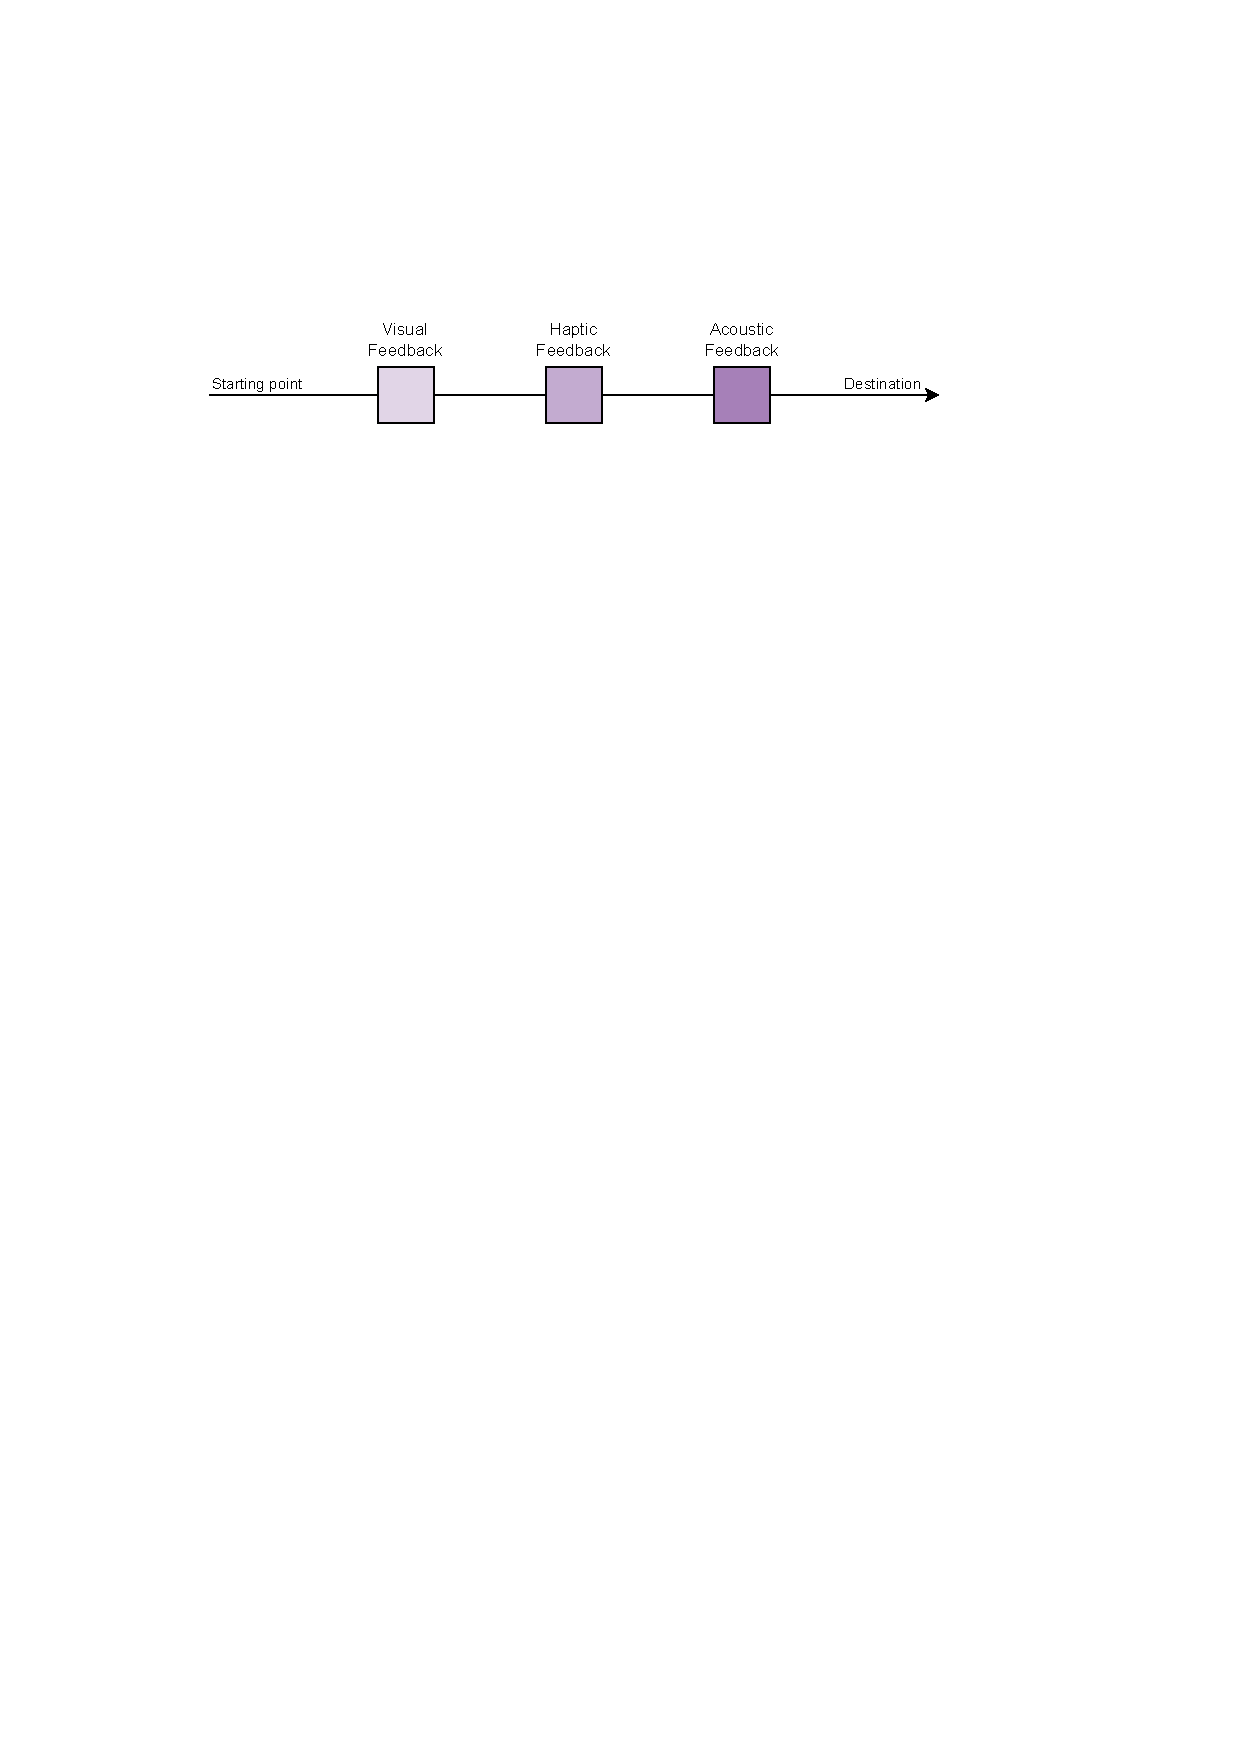
\includegraphics[width=14cm]{Perlenkette.pdf}}}%
    \qquad
    \subfloat[\centering]{{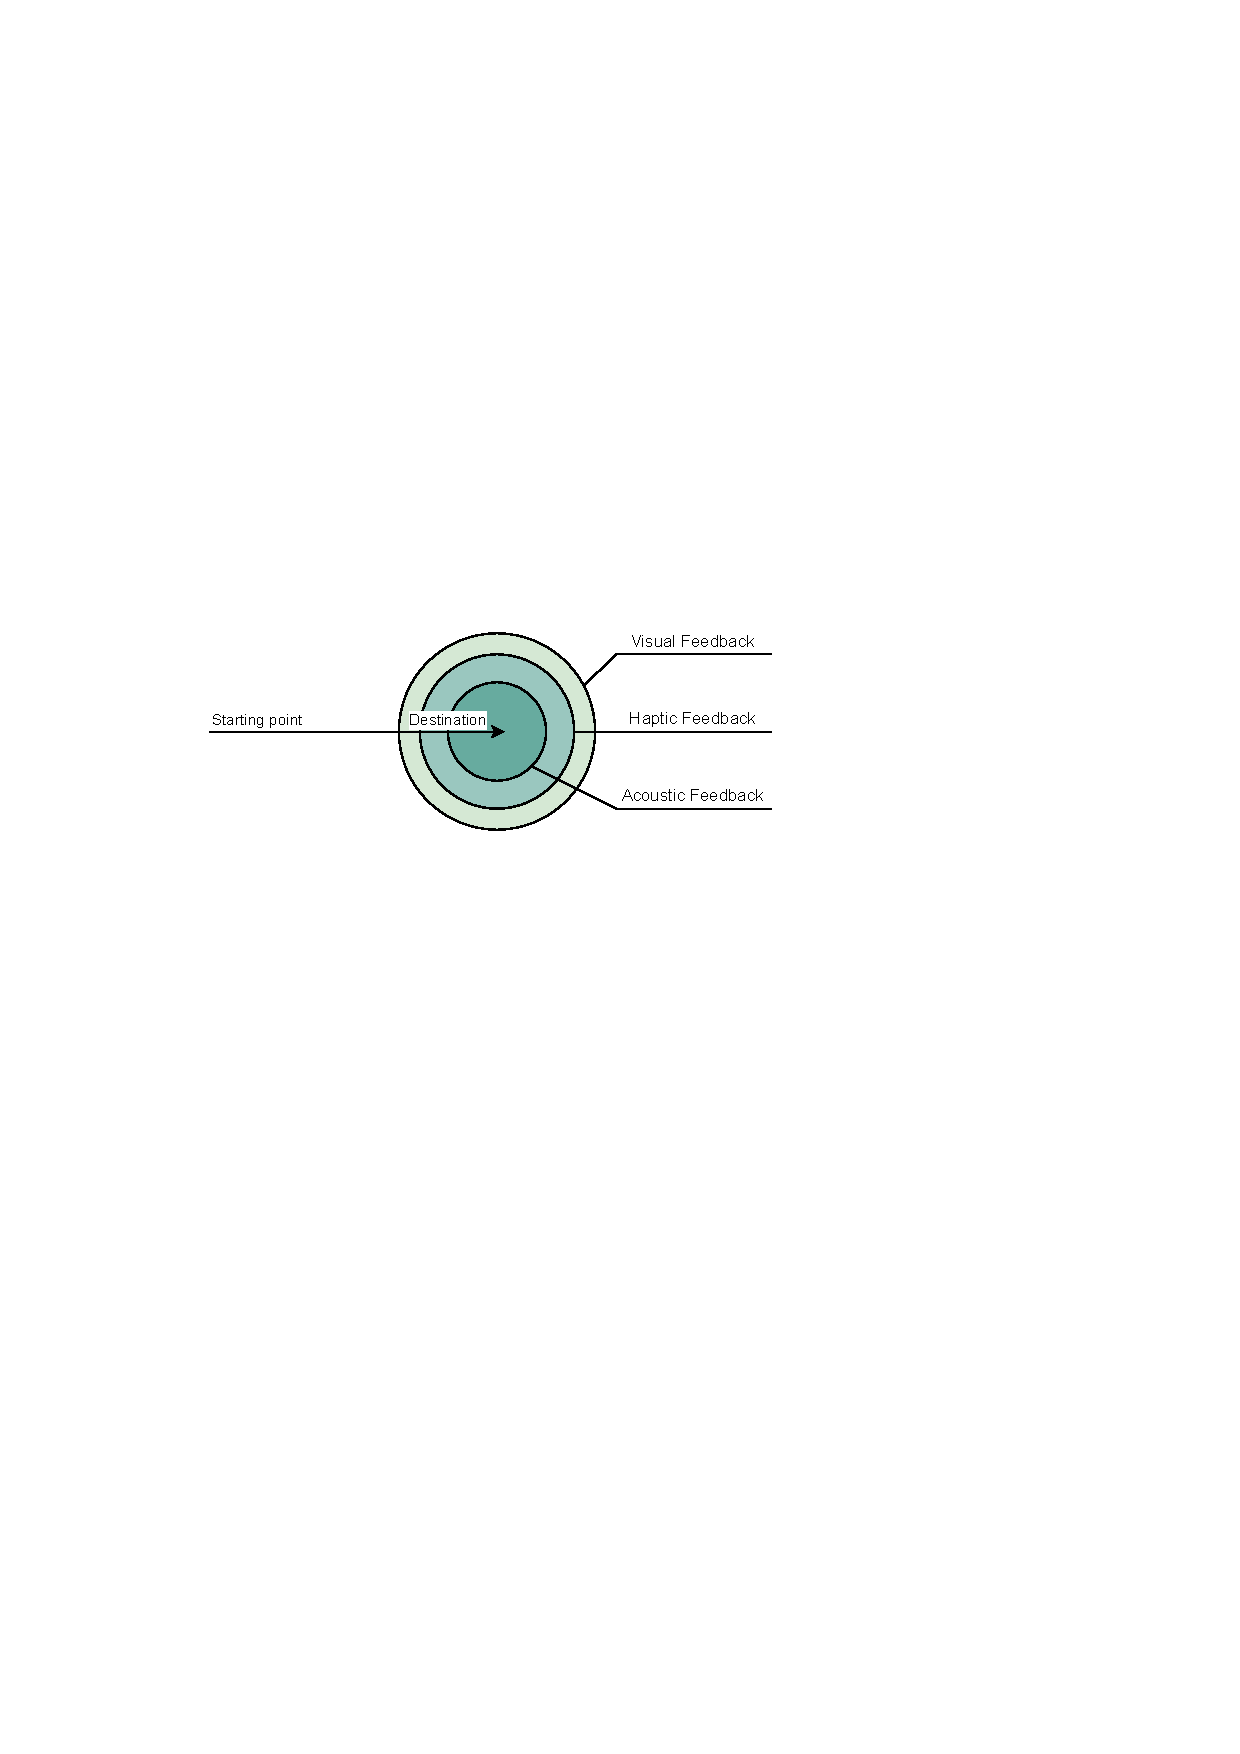
\includegraphics[width=12cm]{Zwiebel.pdf}}}%
    \caption{Escalation of reminders following a sequential model (a) and a concentric model (b)}%
    \label{fig:reminderescalation}%
\end{figure}

\subsection{Triggers}
Beyond how reminders are structured, it must also be considered how they could be triggered in the first place. 
The timing of these reminders plays an important role in ensuring that users are notified at the right moment during their journey. 
Different approaches could be explored, depending on whether reminders should be based on time, location or distance to the destination.

One possible approach would be to rely on fixed arrival times, where reminders could be triggered at predefined intervals before reaching the stop.
This would ensure that users receive alerts at specific time points, regardless of external factors such as travel speed or delays. 
Another option could be to determine triggers based on the user's location along the route, so that reminders are activated as they move closer to their destination. 
Unlike the time-based approach, this method would not depend on scheduled arrival times but rather on the user's actual position relative to their stop.
These two approaches might follow a sequential model as discussed in Subsection \ref{sec:escalations}, activating reminders at distinct points along the journey. 
Alternatively, a concentric approach could be considered, where reminders are triggered based on distance to the destination, where different zones around the destination are used to trigger reminders at increasing proximity.
In this context, it could be considered whether geofencing might be used to allow the system to detect when the user crosses predefined distance markers.

\section{Data Persistence}
It is being considered that the app will require some form of data persistence to store user data beyond the app's runtime. 
The system envisions two main types of persistent data: user preferences and reminder objects. 
User preferences define how reminders behave, whereas reminder objects should store trip-related details.
While the concept foresees that users can configure preferences for each reminder individually, there is also the idea that frequently used settings could be saved and easily reapplied.
The following subsections outline these data structures in more detail.

\subsection{User Preferences}
For user preferences, it is being considered that the reminder behavior, whether time-based or location-based, could be represented through a mode variable that is then stored in a database.
Additionally, an interval setting could define when the user receives reminders, depending on the selected mode. 
For example, if reminders are scheduled in a time-based manner, one possible approach could be to define the interval in minutes before arrival at the destination, such as triggering a reminder five minutes before.
In the case of a location-based mode, the interval could instead be expressed in proximity, for instance 500 meters before reaching the destination.
Furthermore, in alignment with the escalating reminder behavior, reminders could appear in different forms. 
These could be visual, haptic, acoustic, or a combination of them. 
However, if a user prefers only a non-intrusive visual cue such as a notification, the app would need to account for this preference to avoid unwanted alerts.
All of these user preference settings would need to be stored to remain consistent beyond the app's runtime.

\subsection{Reminders}
When it comes to the reminder object itself, several parameters would need to be considered.
The required information depends on whether the user prefers time-based or location-based reminders.
For a time-based reminder, storing a specific time and date would be essential.
For a location-based reminder, the system would need to store the latitude and longitude of the destination.
This should allow the user's current position to be compared against the target location, ensuring the reminder is triggered at the right moment.
Additionally, the names of the starting and destination stations should be stored for display in an overview of active reminders.
The approach also aims to allow unscheduling of reminders, requiring each reminder object to have a unique identifier to locate the correct object and modify it.